\section{Inertiale Messeinheit}
\label{sec:IMU}
Um die benötigte Beschleunigung entlang der x- und y-Achse und die Neigung um die x-, y- und z-Achse, zu erfassen muss ein geeigneter Sensor verwendet werden. Wie in Sektion \ref{subsec:tIMU} beschrieben, handelt es bei einer IMU um eine Kombination aus Accelerometern, Gyroskopen und Magnetometern, die zur Bestimmung von Beschleunigungen und Lage im dreidimensionalen Raum verwendet wird. Somit kann eine IMU alle oben erwähnten Werte erfassen und bereitstellen, deswegen eignet sie sich perfekt für das ferngesteuerte Auto.
\subsection{Wahl der inertialen Messeinheit}
\label{subsec:IMUchoice}
Es gibt viele \ac{IMU}'s, die sich für die Verwendung mit dem Raspberry Pi eignen, die am Weitesten verbreiteten Modelle sind aber der MPU6050, der MPU9250 und der BNO055. Beim Vergleich dieser Sensoren fällt auf, dass jeder eigene Vor- und Nachteile hat. 
\begin{table}[h]
\centering
\begin{tabular}{|c||c|c|c|} 
\hline
IMU              & MPU6050                                                                      & MPU9250                                                                                    & BNO055                                                                                      \\ 
\hhline{|=::===|}
Sensoren         & \begin{tabular}[c]{@{}c@{}}Accelerometer\\Gyroskop\\Thermometer\end{tabular} & \begin{tabular}[c]{@{}c@{}}Accelerometer\\Gyroskop\\Magnetometer\\Thermometer\end{tabular} & \begin{tabular}[c]{@{}c@{}}Accelerometer\\Gyroskop\\Magnetometer\\Thermometer\end{tabular}  \\ 
\hline
Freiheitsgrade   & 6                                                                            & 9                                                                                          & 9                                                                                           \\ 
\hline
Zusatzfunktionen & -                                                                            & -                                                                                          & Integrierte Sensorfusion                                                                    \\ 
\hline
Preis            & $\sim$5\officialeuro                                                          & $\sim$11\officialeuro                                                                       & $\sim$35\officialeuro                                                                       \\
\hline
\end{tabular}
\caption{Vergleich von MPU6050, MPU9250 \& BNO055}
\label{tab:IMUcomparison}
\end{table}
\\
Aufgrund des inkludierten Magnetometers und dem im Vergleich zum BNO055 niedrigen Preis wird der MPU9250 verwendet. Da diese \ac{IMU} selbst keine Sensorfusion durchführen kann, muss diese auf dem Raspberry Pi stattfinden.

\subsection{Montage der inertialen Messeinheit}
\label{subsec:IMUmount}
Um eine korrekte Erfassung der Messdaten zu gewährleisten muss der MPU9250 mittig entlang der Drehachse in Fahrtrichtung angebracht werden. Dazu wird eine Montage-Vorrichtung mithilfe von \ac{CAD} konstruiert und anschließend per \ac{DUP}-3D-Druck gefertigt. Die Platine ist mit zwei M3 Schrauben in diesem Gehäuse befestigt (Siehe Abbildung \ref{fig:MPUmount}). Um die Aufzeichnung von feinen Vibrationen zu vermindern, wird die Halterung mit Silikondämpfern im Gehäuse der Elektronik befestigt. 
\begin{figure}[h]
\centering
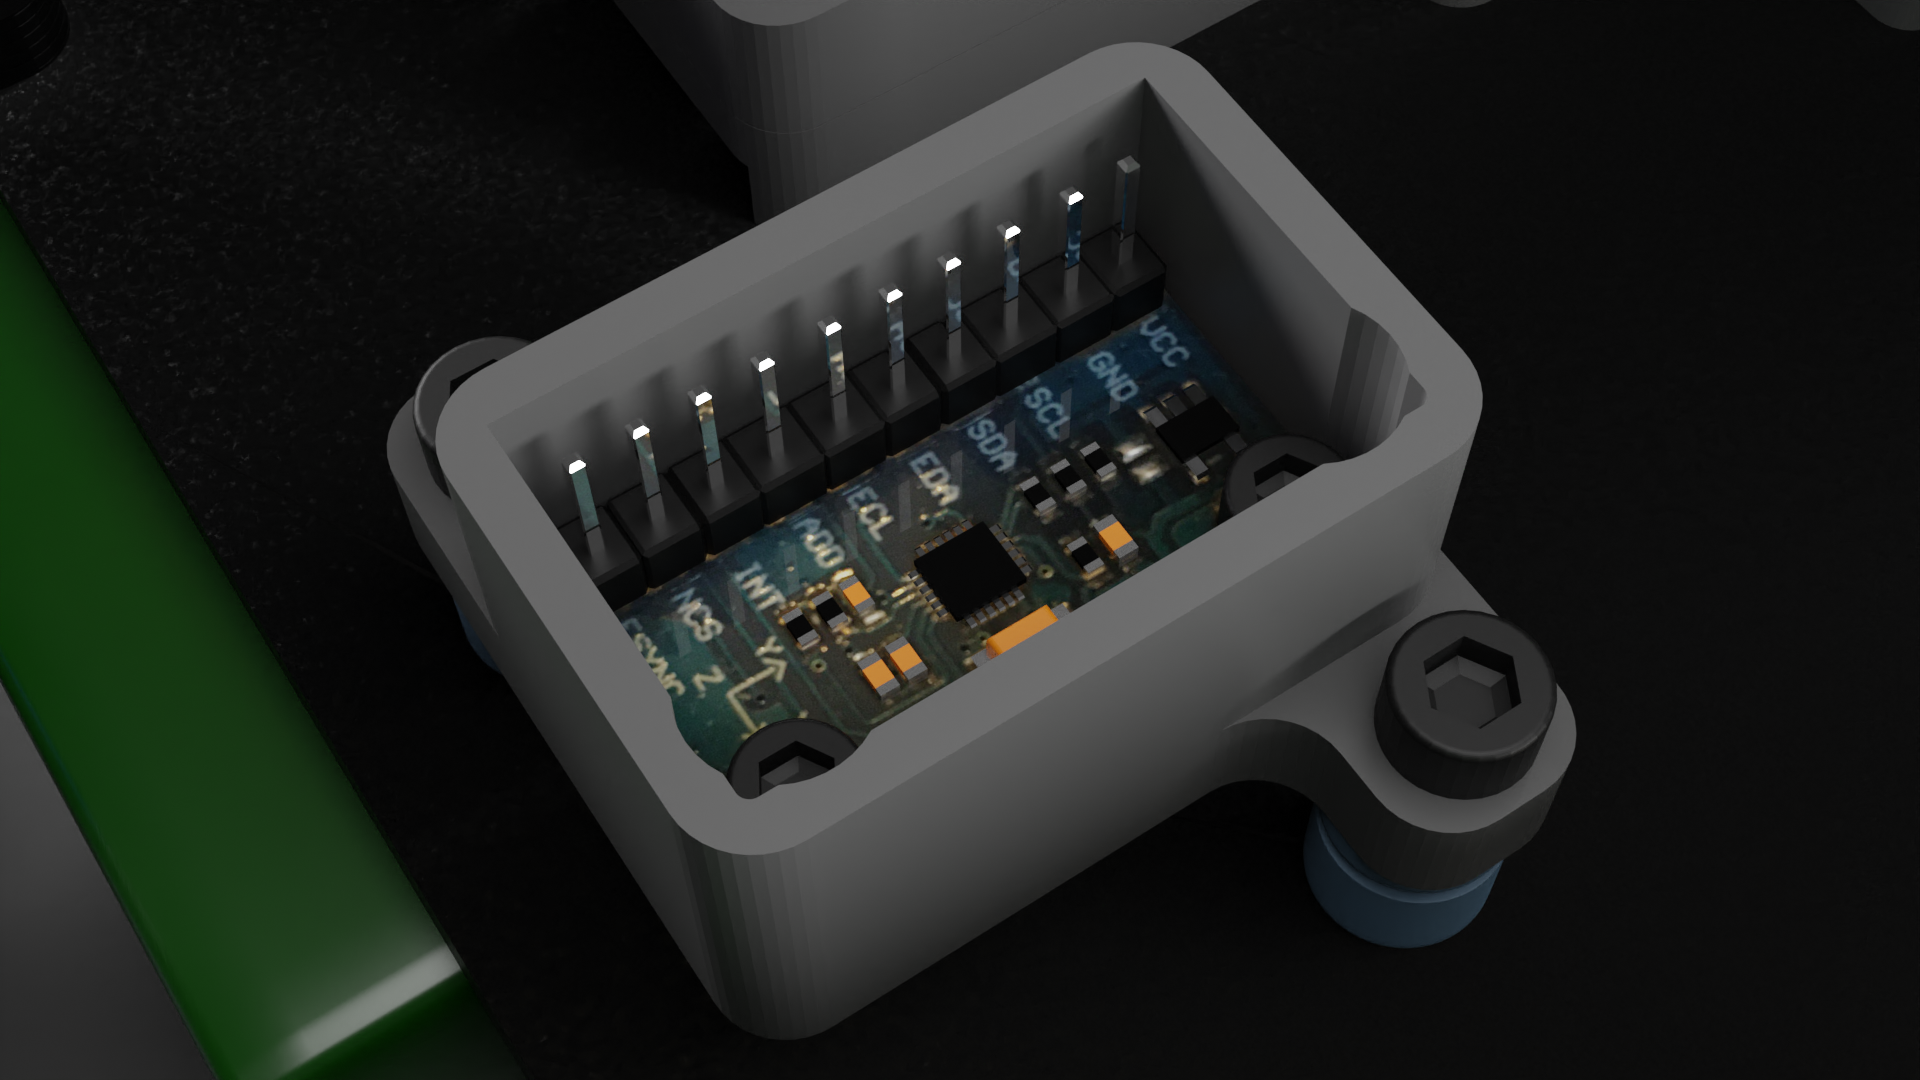
\includegraphics[scale=0.2]{MPUmount.png}
\caption{Montage des MPU9250 im Gehäuse}
\label{fig:MPUmount}
\end{figure}

\subsection{Programmatische Implementation der inertialen Messeinheit}
\label{subsec:IMUprogram}
Der MPU9250 stellt die gemessenen Werte über den \ac{I2C} Bus bereit. Um diese Werte mit Python am Raspberry Pi auslesen zu können, kann die Bibliothek \glqq smbus\grqq \ (\url{https://pypi.org/project/smbus/}) verwendet werden. Smbus ist eine Python-Implementation der i2c-tools für den Linux-Kernel. Mithilfe von smbus und der \ac{I2C}-Adresse des Sensors können die gemessenen Werte aus den jeweiligen Registern entnommen werden. Diese Werte enthalten aber noch die Erdbeschleunigung und stellen noch keine Lage dar. Um eine zuverlässige Bestimmung der Lage im dreidimensionalen Raum zu ermöglichen, muss wie in Sektion \ref{subsec:tIMU} beschrieben Sensorfusion betrieben werden. Für die einfache Implementation dieses Prozesses gibt es die in Sektion \ref{subsubsec:tLibImusensor} beschriebene Python-Bibliothek \glqq imusensor\grqq . Da der Raspberry Pi den benötigten Rechenaufwand für Madgwick problemlos aufbringen kann, wird in diesem Fall Madgwick verwendet. \\
Diese Werte beinhalten aber noch immer die Erdanziehungskraft, was in Fällen, in denen sich das ferngesteuerte Auto nicht in einer horizontalen Lage befindet die Messwerte in x- und y-Richtung beeinflusst. Um dieses Problem zu lösen kann mithilfe der Lage im Raum bestimmt werden, auf welche Achse welcher Anteil der Erdbeschleunigung  wirkt. Die dafür benötigten Formeln können aus den Winkelfunktionen abgeleitet werden.
Die abgeleiteten Formeln für die Beschleunigung in x- (\ref{eqn:imuFx}), y- (\ref{eqn:imuFy}) und z-Richtung (\ref{eqn:imuFz}) sind unten zu sehen.
\begin{equation}
Ax=\frac{g*\tan(\gamma)}{\sqrt{\frac{\tan(\gamma)^2}{\cos(\beta)^2}+1}}
\label{eqn:imuFx}
\end{equation}

\begin{equation}
Ay=\frac{g}{\sqrt{\tan(\gamma)^2+\tan(\alpha)^2+1}}
\label{eqn:imuFy}
\end{equation}

\begin{equation}
Az=\frac{g}{\sqrt{\cot(\alpha)^2+\cot(\beta)^2+1}}
\label{eqn:imuFz}
\end{equation}

Dabei stellt g die Erdbeschleunigung, $\alpha$ die Rotation um die x-Achse (roll), $\beta$ die Rotation um die y-Achse (pitch) und $\gamma$ die Rotation um die z-Achse (yaw) dar. \\
Um festzustellen, ob der jeweilige Anteil der Erdbeschleunigung subtrahiert oder addiert werden muss, können roll und pitch des Autos betrachtet werden. Wenn sich das Auto in einer horizontalen Lage befindet, ist sowohl roll als auch pitch null. Wenn sich das Auto nach links neigt, wird roll negativ, sollte es sich nach rechts neigen, wird roll positiv. Dasselbe gilt auch für pitch, neigt sich das Auto nach vorne, wird pitch negativ und vice versa. Solange roll also kleiner als null ist, muss das Offset in y-Richtung addiert werden, sollte roll größer als null sein, muss das Offset subtrahiert werden. Dasselbe gilt für pitch und das Offset in x-Richtung. Das Offset in z-Richtung kann immer addiert werden, da das Auto niemals eine Steigung von mehr als $\infty$ bzw. weniger als -$\infty$ befahren kann.

\subsection{Probleme der inertialen Messeinheit}
\label{subsec:IMUproblems}
Trotz der in Sektion \ref{subsec:IMUmount} beschriebenen gedämpften Befestigung der inertialen Messeinheit stellen die durch den Motor und das Getriebe erzeugten Vibrationen ein Problem dar. Da die Elektronik auf derselben Grundplatte wie das Antriebssystem befestigt ist, werden diese Vibrationen direkt von der \ac{IMU} aufgenommen, wodurch die Messwerte verfälscht werden. Diese Verfälschungen sind so stark, dass die Messwerte komplett unbrauchbar sind. Eine theoretische mögliche Lösung für dieses Problem ist es, die Messeinheit noch schwingungsdämpfender zu montieren. 